\documentclass[tikz,border=12pt]{standalone}
\usepackage{amsmath}
\usetikzlibrary{arrows.meta,calc}

\begin{document}
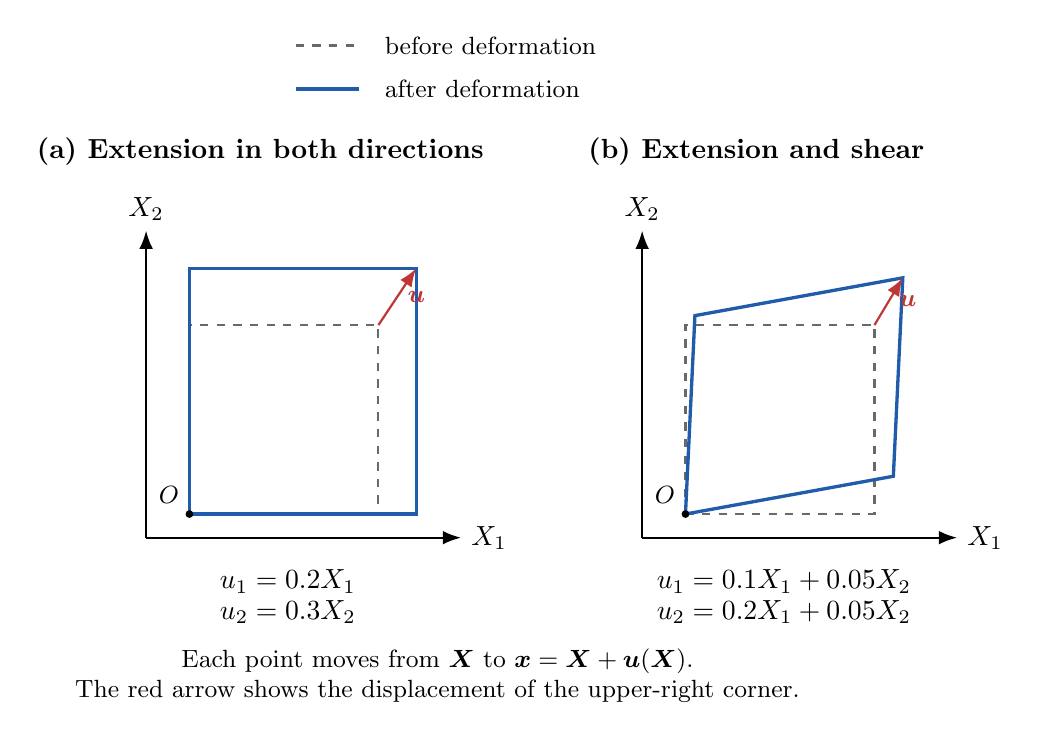
\begin{tikzpicture}[>=Latex,font=\sffamily,thick]
\definecolor{reference}{RGB}{105,105,105}
\definecolor{deformed}{RGB}{32,92,170}
\definecolor{displacement}{RGB}{190,55,55}

% Stack the legend entries so labels cannot overlap adjacent line samples.
\draw[dashed,reference] (-1.80,5.95)--(-1.00,5.95);
\node[anchor=west,font=\small] at (-0.80,5.95) {before deformation};
\draw[deformed,very thick] (-1.80,5.40)--(-1.00,5.40);
\node[anchor=west,font=\small] at (-0.80,5.40) {after deformation};

% (a) u1 = 0.2 x1, u2 = 0.3 x2.
\begin{scope}[shift={(-3.15,0)}]
  \node[font=\bfseries] at (0.9,4.60) {(a) Extension in both directions};
  \draw[->] (-0.55,-0.30)--(3.45,-0.30) node[right] {$X_1$};
  \draw[->] (-0.55,-0.30)--(-0.55,3.60) node[above] {$X_2$};
  \coordinate (A) at (0,0);
  \coordinate (B) at (2.4,0);
  \coordinate (C) at (2.4,2.4);
  \coordinate (D) at (0,2.4);
  \coordinate (Bp) at (2.88,0);
  \coordinate (Cp) at (2.88,3.12);
  \coordinate (Dp) at (0,3.12);
  \draw[dashed,reference] (A)--(B)--(C)--(D)--cycle;
  \draw[deformed,very thick] (A)--(Bp)--(Cp)--(Dp)--cycle;
  \draw[->,displacement] (C)--(Cp)
    node[midway,right,font=\small] {$\boldsymbol u$};
  \fill (A) circle (1.4pt) node[above left,font=\small] {$O$};
  \node[align=center] at (1.25,-1.05)
    {$u_1=0.2X_1$\\[-1pt]$u_2=0.3X_2$};
\end{scope}

% (b) u1 = 0.1 x1 + 0.05 x2, u2 = 0.2 x1 + 0.05 x2.
\begin{scope}[shift={(3.15,0)}]
  \node[font=\bfseries] at (0.9,4.60) {(b) Extension and shear};
  \draw[->] (-0.55,-0.30)--(3.45,-0.30) node[right] {$X_1$};
  \draw[->] (-0.55,-0.30)--(-0.55,3.60) node[above] {$X_2$};
  \coordinate (A) at (0,0);
  \coordinate (B) at (2.4,0);
  \coordinate (C) at (2.4,2.4);
  \coordinate (D) at (0,2.4);
  % x = X + u(X) = [[1.1, 0.05], [0.2, 1.05]] X.
  \coordinate (Bp) at (2.64,0.48);
  \coordinate (Cp) at (2.76,3.00);
  \coordinate (Dp) at (0.12,2.52);
  \draw[dashed,reference] (A)--(B)--(C)--(D)--cycle;
  \draw[deformed,very thick] (A)--(Bp)--(Cp)--(Dp)--cycle;
  \draw[->,displacement] (C)--(Cp)
    node[midway,right,font=\small] {$\boldsymbol u$};
  \fill (A) circle (1.4pt) node[above left,font=\small] {$O$};
  \node[align=center] at (1.25,-1.05)
    {$u_1=0.1X_1+0.05X_2$\\[-1pt]$u_2=0.2X_1+0.05X_2$};
\end{scope}

\node[align=center,font=\small] at (0,-2.05)
  {Each point moves from $\boldsymbol X$ to $\boldsymbol x=\boldsymbol X+\boldsymbol u(\boldsymbol X)$.\\
   The red arrow shows the displacement of the upper-right corner.};
\end{tikzpicture}
\end{document}
